\begin{figure}[ht]
  \centering
  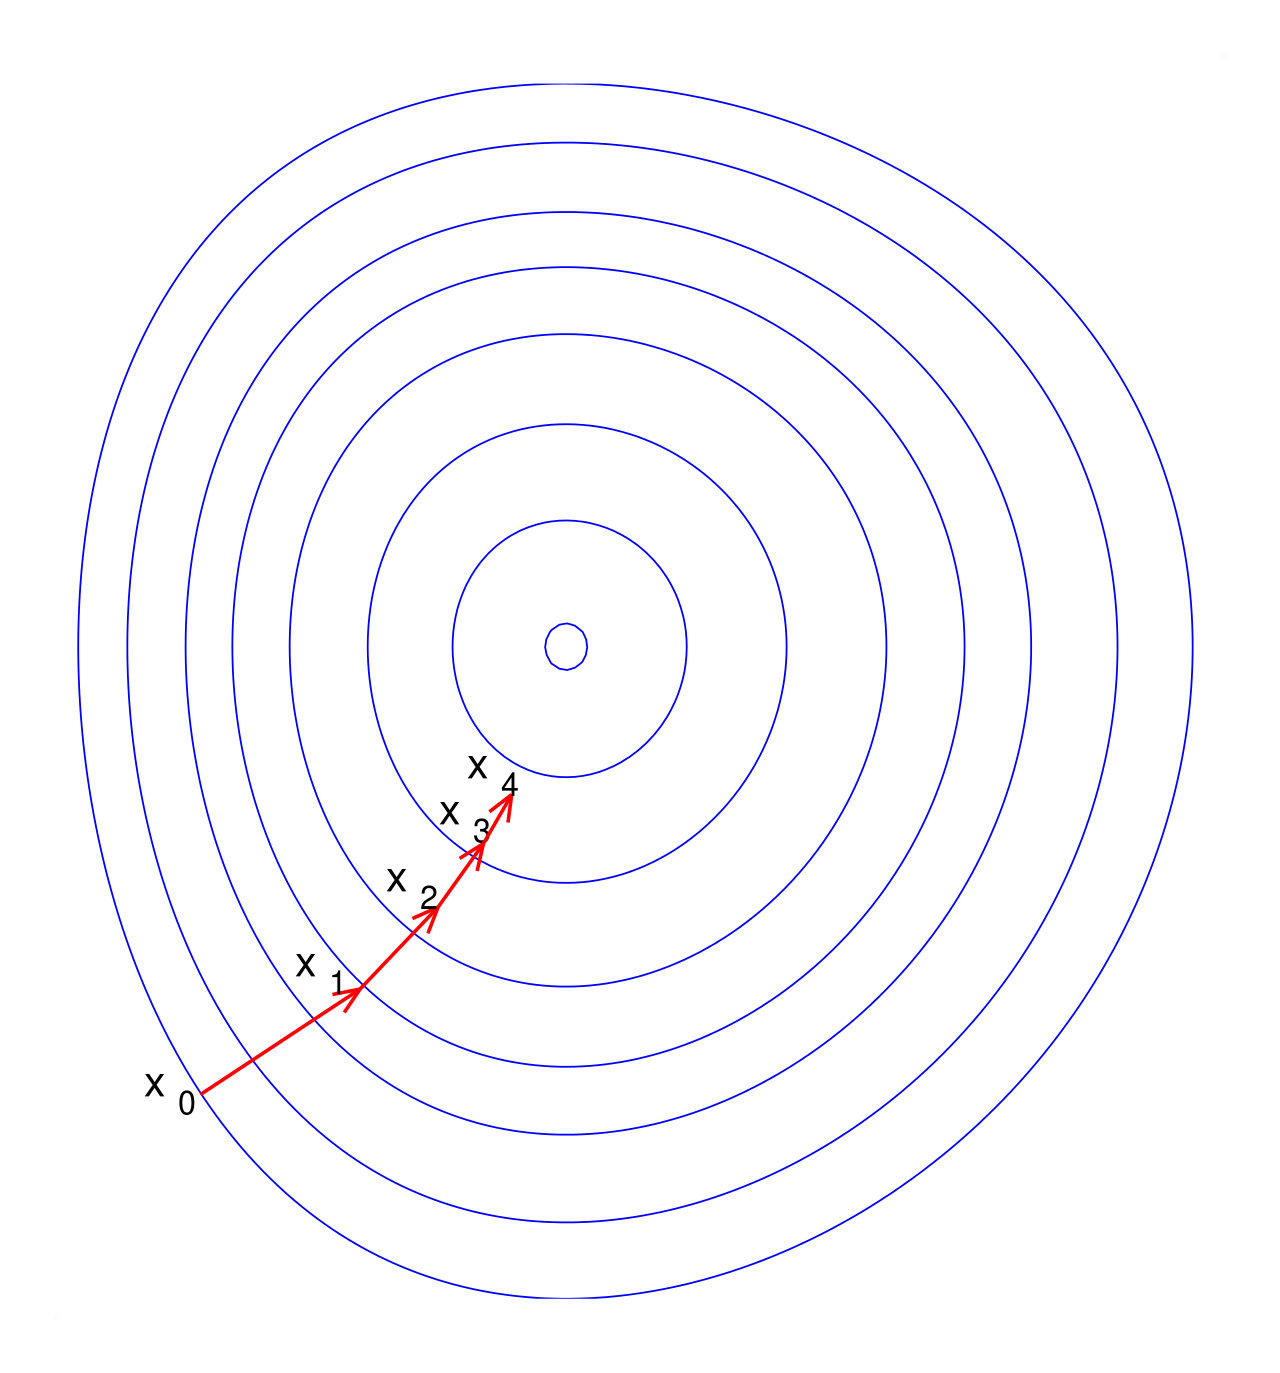
\includegraphics[width=.6\textwidth]{gradient-descent}
  \caption{An illustration of the gradient descent algorithm. The blue lines
    represent level sets of a function, sets of points that have the same
    gradient. The $x$'s represent where in along the function the algorithm is
    at a given step with the steps numbered 0 to 4.}
  \label{fig:quadrupole}
\end{figure}
  